\documentclass{standalone}
\usepackage{tikz}
\usetikzlibrary{patterns}
\usetikzlibrary{positioning}
\usetikzlibrary{patterns, positioning}
\usetikzlibrary{shapes.misc}
\usepackage[outline]{contour}
\contourlength{1.5pt} 
\usetikzlibrary{calc}
        \usepackage{relsize}
        \tikzset{fontscale/.style = {font=\relsize{#1}}}

\begin{document}
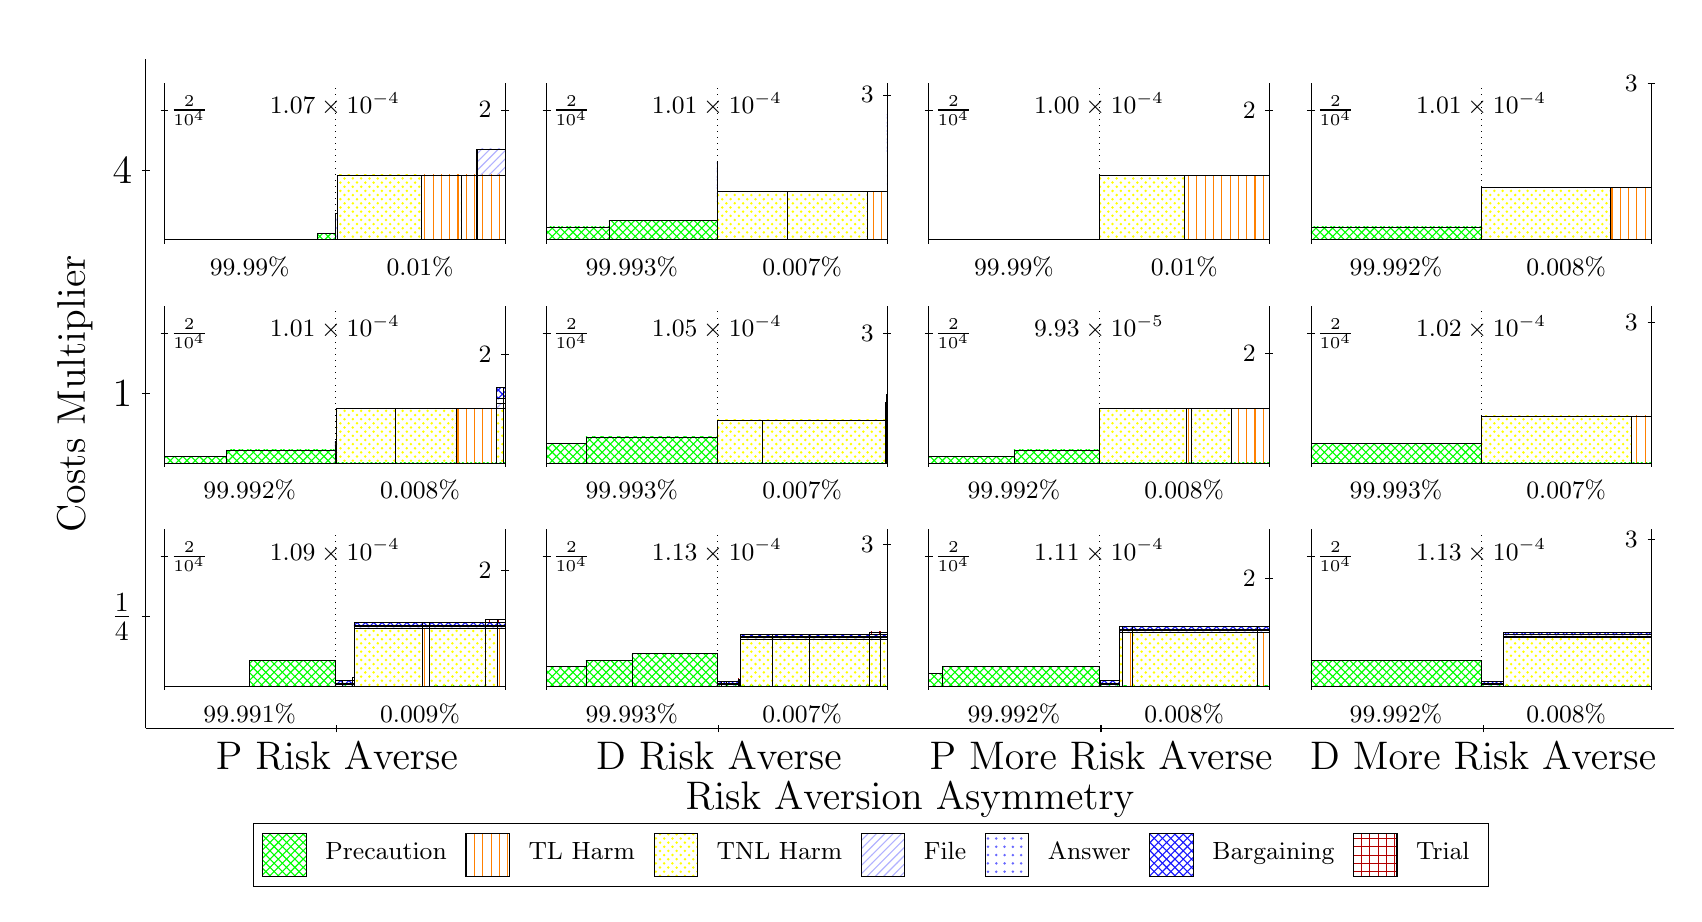
\begin{tikzpicture}
\clip(-0.5,-1.1) rectangle +(20.91,11);
\draw[black] (1,1) -- (1,9.5);
\node[rotate=90, fontscale=2, anchor=center] at (0.1, 5.25) {Costs Multiplier};
\draw[black] (0.95,2.4167) -- (1.05,2.4167);
\node[fontscale=2, anchor=east] at (0.95, 2.4167) {$\frac{1}{4}$};
\draw[black] (0.95,5.25) -- (1.05,5.25);
\node[fontscale=2, anchor=east] at (0.95, 5.25) {1};
\draw[black] (0.95,8.0833) -- (1.05,8.0833);
\node[fontscale=2, anchor=east] at (0.95, 8.0833) {4};

\draw[black] (1,1) -- (20.41,1);
\node[fontscale=2, anchor=center] at (10.705, 0.1) {Risk Aversion Asymmetry};
\draw[black] (3.4263,0.95) -- (3.4263,1.05);
\node[fontscale=2, anchor=north] at (3.4263, 0.95) {P Risk Averse};
\draw[black] (8.2788,0.95) -- (8.2788,1.05);
\node[fontscale=2, anchor=north] at (8.2788, 0.95) {D Risk Averse};
\draw[black] (13.131,0.95) -- (13.131,1.05);
\node[fontscale=2, anchor=north] at (13.131, 0.95) {P More Risk Averse};
\draw[black] (17.984,0.95) -- (17.984,1.05);
\node[fontscale=2, anchor=north] at (17.984, 0.95) {D More Risk Averse};


\draw[pattern=crosshatch, pattern color=green,draw=black,very thin] (2.3197,1.54) rectangle (3.4013,1.8686);
\draw[pattern=north east lines, pattern color=blue!30,draw=black,very thin] (3.4013,1.54) rectangle (3.4967,1.5583);
\draw[pattern=dots,  pattern color=blue!60,draw=black,very thin] (3.4013,1.5583) rectangle (3.4967,1.5767);
\draw[pattern=crosshatch,      pattern color=blue!90,draw=black,very thin] (3.4013,1.5767) rectangle (3.4967,1.6134);
\draw[pattern=crosshatch, pattern color=green,draw=black,very thin] (3.4967,1.54) rectangle (3.6184,1.54);
\draw[pattern=north east lines, pattern color=blue!30,draw=black,very thin] (3.4967,1.54) rectangle (3.6184,1.5584);
\draw[pattern=dots,  pattern color=blue!60,draw=black,very thin] (3.4967,1.5584) rectangle (3.6184,1.5767);
\draw[pattern=crosshatch,      pattern color=blue!90,draw=black,very thin] (3.4967,1.5767) rectangle (3.6184,1.6134);
\draw[pattern=north east lines, pattern color=blue!30,draw=black,very thin] (3.6184,1.54) rectangle (3.6441,1.5583);
\draw[pattern=dots,  pattern color=blue!60,draw=black,very thin] (3.6184,1.5583) rectangle (3.6441,1.5767);
\draw[pattern=crosshatch,      pattern color=blue!90,draw=black,very thin] (3.6184,1.5767) rectangle (3.6441,1.6134);
\draw[pattern=grid,            pattern color=red!70!black,draw=black,very thin] (3.6184,1.6134) rectangle (3.6441,1.6501);
\draw[pattern=crosshatch dots, pattern color=yellow,draw=black,very thin] (3.6441,1.54) rectangle (4.5104,2.2738);
\draw[pattern=north east lines, pattern color=blue!30,draw=black,very thin] (3.6441,2.2738) rectangle (4.5104,2.2921);
\draw[pattern=dots,  pattern color=blue!60,draw=black,very thin] (3.6441,2.2921) rectangle (4.5104,2.3105);
\draw[pattern=crosshatch,      pattern color=blue!90,draw=black,very thin] (3.6441,2.3105) rectangle (4.5104,2.3472);
\draw[pattern=vertical lines, pattern color=orange,draw=black,very thin] (4.5104,1.54) rectangle (4.5983,2.2738);
\draw[pattern=north east lines, pattern color=blue!30,draw=black,very thin] (4.5104,2.2738) rectangle (4.5983,2.2921);
\draw[pattern=dots,  pattern color=blue!60,draw=black,very thin] (4.5104,2.2921) rectangle (4.5983,2.3105);
\draw[pattern=crosshatch,      pattern color=blue!90,draw=black,very thin] (4.5104,2.3105) rectangle (4.5983,2.3472);
\draw[pattern=crosshatch, pattern color=green,draw=black,very thin] (4.5983,1.54) rectangle (5.3076,1.54);
\draw[pattern=crosshatch dots, pattern color=yellow,draw=black,very thin] (4.5983,1.54) rectangle (5.3076,2.2738);
\draw[pattern=north east lines, pattern color=blue!30,draw=black,very thin] (4.5983,2.2738) rectangle (5.3076,2.2922);
\draw[pattern=dots,  pattern color=blue!60,draw=black,very thin] (4.5983,2.2922) rectangle (5.3076,2.3105);
\draw[pattern=crosshatch,      pattern color=blue!90,draw=black,very thin] (4.5983,2.3105) rectangle (5.3076,2.3472);
\draw[pattern=crosshatch dots, pattern color=yellow,draw=black,very thin] (5.3076,1.54) rectangle (5.4655,2.2738);
\draw[pattern=north east lines, pattern color=blue!30,draw=black,very thin] (5.3076,2.2738) rectangle (5.4655,2.2921);
\draw[pattern=dots,  pattern color=blue!60,draw=black,very thin] (5.3076,2.2921) rectangle (5.4655,2.3105);
\draw[pattern=crosshatch,      pattern color=blue!90,draw=black,very thin] (5.3076,2.3105) rectangle (5.4655,2.3472);
\draw[pattern=grid,            pattern color=red!70!black,draw=black,very thin] (5.3076,2.3472) rectangle (5.4655,2.3839);
\draw[pattern=vertical lines, pattern color=orange,draw=black,very thin] (5.4655,1.54) rectangle (5.5644,2.2738);
\draw[pattern=north east lines, pattern color=blue!30,draw=black,very thin] (5.4655,2.2738) rectangle (5.5644,2.2921);
\draw[pattern=dots,  pattern color=blue!60,draw=black,very thin] (5.4655,2.2921) rectangle (5.5644,2.3105);
\draw[pattern=crosshatch,      pattern color=blue!90,draw=black,very thin] (5.4655,2.3105) rectangle (5.5644,2.3472);
\draw[pattern=grid,            pattern color=red!70!black,draw=black,very thin] (5.4655,2.3472) rectangle (5.5644,2.3839);
\node[font=\small,text=black,anchor=north] at (3.4013, 3.5333) {$1.09\times 10^{-4}$};
\draw[black,very thin] (1.2381,1.54) -- (1.2381,3.5333);
\draw[black,very thin] (1.1881,3.1831) -- (1.2881,3.1831);
\node[font=\small,text=black, anchor=west] at (1.1881, 3.1831) {$\frac{2}{10^{4}}$};

\draw[black,dotted,very thin] (3.4013,1.5998) -- (3.4013,3.4735);
\draw[black,very thin] (5.5644,1.54) -- (5.5644,3.5333);
\draw[black,very thin] (5.5144,3.0076) -- (5.6144,3.0076);
\node[font=\small,text=black, anchor=east] at (5.5144, 3.0076) {\contour{white}{2}};

\draw[black,very thin] (1.2381,1.54) -- (5.5644,1.54);
\draw[black,very thin] (1.2381,1.49) -- (1.2381,1.59);
\node[font=\small,text=black, anchor=north] at (1.2381, 1.49) {};
\draw[black,very thin] (5.5644,1.49) -- (5.5644,1.59);
\node[font=\small,text=black, anchor=north] at (5.5644, 1.49) {};

\node[font=\small,text=black,anchor=south] at (2.3197, 0.94) {99.991\%};
\node[font=\small,text=black,anchor=south] at (4.4828, 0.94) {0.009\%};

\draw[pattern=crosshatch, pattern color=green,draw=black,very thin] (6.0906,1.54) rectangle (6.5882,1.7865);
\draw[pattern=crosshatch, pattern color=green,draw=black,very thin] (6.5882,1.54) rectangle (7.1722,1.8686);
\draw[pattern=crosshatch, pattern color=green,draw=black,very thin] (7.1722,1.54) rectangle (8.2538,1.9508);
\draw[pattern=crosshatch, pattern color=green,draw=black,very thin] (8.2538,1.54) rectangle (8.3038,1.54);
\draw[pattern=north east lines, pattern color=blue!30,draw=black,very thin] (8.2538,1.54) rectangle (8.3038,1.555);
\draw[pattern=dots,  pattern color=blue!60,draw=black,very thin] (8.2538,1.555) rectangle (8.3038,1.5699);
\draw[pattern=crosshatch,      pattern color=blue!90,draw=black,very thin] (8.2538,1.5699) rectangle (8.3038,1.5998);
\draw[pattern=crosshatch, pattern color=green,draw=black,very thin] (8.3038,1.54) rectangle (8.3684,1.54);
\draw[pattern=north east lines, pattern color=blue!30,draw=black,very thin] (8.3038,1.54) rectangle (8.3684,1.555);
\draw[pattern=dots,  pattern color=blue!60,draw=black,very thin] (8.3038,1.555) rectangle (8.3684,1.5699);
\draw[pattern=crosshatch,      pattern color=blue!90,draw=black,very thin] (8.3038,1.5699) rectangle (8.3684,1.5998);
\draw[pattern=crosshatch, pattern color=green,draw=black,very thin] (8.3684,1.54) rectangle (8.5182,1.54);
\draw[pattern=north east lines, pattern color=blue!30,draw=black,very thin] (8.3684,1.54) rectangle (8.5182,1.555);
\draw[pattern=dots,  pattern color=blue!60,draw=black,very thin] (8.3684,1.555) rectangle (8.5182,1.5699);
\draw[pattern=crosshatch,      pattern color=blue!90,draw=black,very thin] (8.3684,1.5699) rectangle (8.5182,1.5998);
\draw[pattern=crosshatch, pattern color=green,draw=black,very thin] (8.5182,1.54) rectangle (8.5362,1.54);
\draw[pattern=north east lines, pattern color=blue!30,draw=black,very thin] (8.5182,1.54) rectangle (8.5362,1.555);
\draw[pattern=dots,  pattern color=blue!60,draw=black,very thin] (8.5182,1.555) rectangle (8.5362,1.5699);
\draw[pattern=crosshatch,      pattern color=blue!90,draw=black,very thin] (8.5182,1.5699) rectangle (8.5362,1.5998);
\draw[pattern=grid,            pattern color=red!70!black,draw=black,very thin] (8.5182,1.5998) rectangle (8.5362,1.6297);
\draw[pattern=crosshatch, pattern color=green,draw=black,very thin] (8.5362,1.54) rectangle (8.5516,1.54);
\draw[pattern=north east lines, pattern color=blue!30,draw=black,very thin] (8.5362,1.54) rectangle (8.5516,1.555);
\draw[pattern=dots,  pattern color=blue!60,draw=black,very thin] (8.5362,1.555) rectangle (8.5516,1.5699);
\draw[pattern=crosshatch,      pattern color=blue!90,draw=black,very thin] (8.5362,1.5699) rectangle (8.5516,1.5998);
\draw[pattern=grid,            pattern color=red!70!black,draw=black,very thin] (8.5362,1.5998) rectangle (8.5516,1.6297);
\draw[pattern=crosshatch, pattern color=green,draw=black,very thin] (8.5516,1.54) rectangle (8.9606,1.54);
\draw[pattern=crosshatch dots, pattern color=yellow,draw=black,very thin] (8.5516,1.54) rectangle (8.9606,2.1379);
\draw[pattern=north east lines, pattern color=blue!30,draw=black,very thin] (8.5516,2.1379) rectangle (8.9606,2.1528);
\draw[pattern=dots,  pattern color=blue!60,draw=black,very thin] (8.5516,2.1528) rectangle (8.9606,2.1677);
\draw[pattern=crosshatch,      pattern color=blue!90,draw=black,very thin] (8.5516,2.1677) rectangle (8.9606,2.1976);
\draw[pattern=crosshatch, pattern color=green,draw=black,very thin] (8.9606,1.54) rectangle (9.4216,1.54);
\draw[pattern=crosshatch dots, pattern color=yellow,draw=black,very thin] (8.9606,1.54) rectangle (9.4216,2.1379);
\draw[pattern=north east lines, pattern color=blue!30,draw=black,very thin] (8.9606,2.1379) rectangle (9.4216,2.1528);
\draw[pattern=dots,  pattern color=blue!60,draw=black,very thin] (8.9606,2.1528) rectangle (9.4216,2.1677);
\draw[pattern=crosshatch,      pattern color=blue!90,draw=black,very thin] (8.9606,2.1677) rectangle (9.4216,2.1976);
\draw[pattern=crosshatch, pattern color=green,draw=black,very thin] (9.4216,1.54) rectangle (10.183,1.54);
\draw[pattern=crosshatch dots, pattern color=yellow,draw=black,very thin] (9.4216,1.54) rectangle (10.183,2.1379);
\draw[pattern=north east lines, pattern color=blue!30,draw=black,very thin] (9.4216,2.1379) rectangle (10.183,2.1528);
\draw[pattern=dots,  pattern color=blue!60,draw=black,very thin] (9.4216,2.1528) rectangle (10.183,2.1678);
\draw[pattern=crosshatch,      pattern color=blue!90,draw=black,very thin] (9.4216,2.1678) rectangle (10.183,2.1976);
\draw[pattern=crosshatch, pattern color=green,draw=black,very thin] (10.183,1.54) rectangle (10.322,1.54);
\draw[pattern=crosshatch dots, pattern color=yellow,draw=black,very thin] (10.183,1.54) rectangle (10.322,2.1379);
\draw[pattern=north east lines, pattern color=blue!30,draw=black,very thin] (10.183,2.1379) rectangle (10.322,2.1528);
\draw[pattern=dots,  pattern color=blue!60,draw=black,very thin] (10.183,2.1528) rectangle (10.322,2.1677);
\draw[pattern=crosshatch,      pattern color=blue!90,draw=black,very thin] (10.183,2.1677) rectangle (10.322,2.1976);
\draw[pattern=grid,            pattern color=red!70!black,draw=black,very thin] (10.183,2.1976) rectangle (10.322,2.2275);
\draw[pattern=crosshatch, pattern color=green,draw=black,very thin] (10.322,1.54) rectangle (10.417,1.54);
\draw[pattern=crosshatch dots, pattern color=yellow,draw=black,very thin] (10.322,1.54) rectangle (10.417,2.1379);
\draw[pattern=north east lines, pattern color=blue!30,draw=black,very thin] (10.322,2.1379) rectangle (10.417,2.1528);
\draw[pattern=dots,  pattern color=blue!60,draw=black,very thin] (10.322,2.1528) rectangle (10.417,2.1677);
\draw[pattern=crosshatch,      pattern color=blue!90,draw=black,very thin] (10.322,2.1677) rectangle (10.417,2.1976);
\draw[pattern=grid,            pattern color=red!70!black,draw=black,very thin] (10.322,2.1976) rectangle (10.417,2.2275);
\node[font=\small,text=black,anchor=north] at (8.2538, 3.5333) {$1.13\times 10^{-4}$};
\draw[black,very thin] (6.0906,1.54) -- (6.0906,3.5333);
\draw[black,very thin] (6.0406,3.1832) -- (6.1406,3.1832);
\node[font=\small,text=black, anchor=west] at (6.0406, 3.1832) {$\frac{2}{10^{4}}$};

\draw[black,dotted,very thin] (8.2538,1.5998) -- (8.2538,3.4735);
\draw[black,very thin] (10.417,1.54) -- (10.417,3.5333);
\draw[black,very thin] (10.367,3.3335) -- (10.467,3.3335);
\node[font=\small,text=black, anchor=east] at (10.367, 3.3335) {\contour{white}{3}};

\draw[black,very thin] (6.0906,1.54) -- (10.417,1.54);
\draw[black,very thin] (6.0906,1.49) -- (6.0906,1.59);
\node[font=\small,text=black, anchor=north] at (6.0906, 1.49) {};
\draw[black,very thin] (10.417,1.49) -- (10.417,1.59);
\node[font=\small,text=black, anchor=north] at (10.417, 1.49) {};

\node[font=\small,text=black,anchor=south] at (7.1722, 0.94) {99.993\%};
\node[font=\small,text=black,anchor=south] at (9.3353, 0.94) {0.007\%};

\draw[pattern=crosshatch, pattern color=green,draw=black,very thin] (10.943,1.54) rectangle (11.119,1.7043);
\draw[pattern=crosshatch, pattern color=green,draw=black,very thin] (11.119,1.54) rectangle (13.106,1.7865);
\draw[pattern=crosshatch, pattern color=green,draw=black,very thin] (13.106,1.54) rectangle (13.127,1.54);
\draw[pattern=north east lines, pattern color=blue!30,draw=black,very thin] (13.106,1.54) rectangle (13.127,1.5571);
\draw[pattern=dots,  pattern color=blue!60,draw=black,very thin] (13.106,1.5571) rectangle (13.127,1.5742);
\draw[pattern=crosshatch,      pattern color=blue!90,draw=black,very thin] (13.106,1.5742) rectangle (13.127,1.6084);
\draw[pattern=crosshatch, pattern color=green,draw=black,very thin] (13.127,1.54) rectangle (13.366,1.54);
\draw[pattern=north east lines, pattern color=blue!30,draw=black,very thin] (13.127,1.54) rectangle (13.366,1.5571);
\draw[pattern=dots,  pattern color=blue!60,draw=black,very thin] (13.127,1.5571) rectangle (13.366,1.5742);
\draw[pattern=crosshatch,      pattern color=blue!90,draw=black,very thin] (13.127,1.5742) rectangle (13.366,1.6085);
\draw[pattern=crosshatch, pattern color=green,draw=black,very thin] (13.366,1.54) rectangle (13.396,1.54);
\draw[pattern=crosshatch dots, pattern color=yellow,draw=black,very thin] (13.366,1.54) rectangle (13.396,2.2243);
\draw[pattern=north east lines, pattern color=blue!30,draw=black,very thin] (13.366,2.2243) rectangle (13.396,2.2414);
\draw[pattern=dots,  pattern color=blue!60,draw=black,very thin] (13.366,2.2414) rectangle (13.396,2.2586);
\draw[pattern=crosshatch,      pattern color=blue!90,draw=black,very thin] (13.366,2.2586) rectangle (13.396,2.2928);
\draw[pattern=crosshatch, pattern color=green,draw=black,very thin] (13.396,1.54) rectangle (13.525,1.54);
\draw[pattern=vertical lines, pattern color=orange,draw=black,very thin] (13.396,1.54) rectangle (13.525,2.2243);
\draw[pattern=north east lines, pattern color=blue!30,draw=black,very thin] (13.396,2.2243) rectangle (13.525,2.2414);
\draw[pattern=dots,  pattern color=blue!60,draw=black,very thin] (13.396,2.2414) rectangle (13.525,2.2586);
\draw[pattern=crosshatch,      pattern color=blue!90,draw=black,very thin] (13.396,2.2586) rectangle (13.525,2.2928);
\draw[pattern=crosshatch, pattern color=green,draw=black,very thin] (13.525,1.54) rectangle (15.118,1.54);
\draw[pattern=crosshatch dots, pattern color=yellow,draw=black,very thin] (13.525,1.54) rectangle (15.118,2.2243);
\draw[pattern=north east lines, pattern color=blue!30,draw=black,very thin] (13.525,2.2243) rectangle (15.118,2.2415);
\draw[pattern=dots,  pattern color=blue!60,draw=black,very thin] (13.525,2.2415) rectangle (15.118,2.2586);
\draw[pattern=crosshatch,      pattern color=blue!90,draw=black,very thin] (13.525,2.2586) rectangle (15.118,2.2928);
\draw[pattern=crosshatch, pattern color=green,draw=black,very thin] (15.118,1.54) rectangle (15.269,1.54);
\draw[pattern=vertical lines, pattern color=orange,draw=black,very thin] (15.118,1.54) rectangle (15.269,2.2243);
\draw[pattern=north east lines, pattern color=blue!30,draw=black,very thin] (15.118,2.2243) rectangle (15.269,2.2415);
\draw[pattern=dots,  pattern color=blue!60,draw=black,very thin] (15.118,2.2415) rectangle (15.269,2.2586);
\draw[pattern=crosshatch,      pattern color=blue!90,draw=black,very thin] (15.118,2.2586) rectangle (15.269,2.2928);
\node[font=\small,text=black,anchor=north] at (13.106, 3.5333) {$1.11\times 10^{-4}$};
\draw[black,very thin] (10.943,1.54) -- (10.943,3.5333);
\draw[black,very thin] (10.893,3.1831) -- (10.993,3.1831);
\node[font=\small,text=black, anchor=west] at (10.893, 3.1831) {$\frac{2}{10^{4}}$};

\draw[black,dotted,very thin] (13.106,1.5998) -- (13.106,3.4735);
\draw[black,very thin] (15.269,1.54) -- (15.269,3.5333);
\draw[black,very thin] (15.219,2.9087) -- (15.319,2.9087);
\node[font=\small,text=black, anchor=east] at (15.219, 2.9087) {\contour{white}{2}};

\draw[black,very thin] (10.943,1.54) -- (15.269,1.54);
\draw[black,very thin] (10.943,1.49) -- (10.943,1.59);
\node[font=\small,text=black, anchor=north] at (10.943, 1.49) {};
\draw[black,very thin] (15.269,1.49) -- (15.269,1.59);
\node[font=\small,text=black, anchor=north] at (15.269, 1.49) {};

\node[font=\small,text=black,anchor=south] at (12.025, 0.94) {99.992\%};
\node[font=\small,text=black,anchor=south] at (14.188, 0.94) {0.008\%};

\draw[pattern=crosshatch, pattern color=green,draw=black,very thin] (15.796,1.54) rectangle (17.959,1.8686);
\draw[pattern=crosshatch, pattern color=green,draw=black,very thin] (17.959,1.54) rectangle (18.246,1.54);
\draw[pattern=north east lines, pattern color=blue!30,draw=black,very thin] (17.959,1.54) rectangle (18.246,1.5555);
\draw[pattern=dots,  pattern color=blue!60,draw=black,very thin] (17.959,1.5555) rectangle (18.246,1.571);
\draw[pattern=crosshatch,      pattern color=blue!90,draw=black,very thin] (17.959,1.571) rectangle (18.246,1.6019);
\draw[pattern=crosshatch, pattern color=green,draw=black,very thin] (18.246,1.54) rectangle (20.122,1.54);
\draw[pattern=crosshatch dots, pattern color=yellow,draw=black,very thin] (18.246,1.54) rectangle (20.122,2.1589);
\draw[pattern=north east lines, pattern color=blue!30,draw=black,very thin] (18.246,2.1589) rectangle (20.122,2.1744);
\draw[pattern=dots,  pattern color=blue!60,draw=black,very thin] (18.246,2.1744) rectangle (20.122,2.1899);
\draw[pattern=crosshatch,      pattern color=blue!90,draw=black,very thin] (18.246,2.1899) rectangle (20.122,2.2208);
\node[font=\small,text=black,anchor=north] at (17.959, 3.5333) {$1.13\times 10^{-4}$};
\draw[black,very thin] (15.796,1.54) -- (15.796,3.5333);
\draw[black,very thin] (15.746,3.1832) -- (15.846,3.1832);
\node[font=\small,text=black, anchor=west] at (15.746, 3.1832) {$\frac{2}{10^{4}}$};

\draw[black,dotted,very thin] (17.959,1.5998) -- (17.959,3.4735);
\draw[black,very thin] (20.122,1.54) -- (20.122,3.5333);
\draw[black,very thin] (20.072,3.3967) -- (20.172,3.3967);
\node[font=\small,text=black, anchor=east] at (20.072, 3.3967) {\contour{white}{3}};

\draw[black,very thin] (15.796,1.54) -- (20.122,1.54);
\draw[black,very thin] (15.796,1.49) -- (15.796,1.59);
\node[font=\small,text=black, anchor=north] at (15.796, 1.49) {};
\draw[black,very thin] (20.122,1.49) -- (20.122,1.59);
\node[font=\small,text=black, anchor=north] at (20.122, 1.49) {};

\node[font=\small,text=black,anchor=south] at (16.877, 0.94) {99.992\%};
\node[font=\small,text=black,anchor=south] at (19.04, 0.94) {0.008\%};

\draw[pattern=crosshatch, pattern color=green,draw=black,very thin] (1.2381,4.3733) rectangle (2.0279,4.4555);
\draw[pattern=crosshatch, pattern color=green,draw=black,very thin] (2.0279,4.3733) rectangle (3.4013,4.5376);
\draw[pattern=crosshatch, pattern color=green,draw=black,very thin] (3.4013,4.3733) rectangle (3.4134,4.3733);
\draw[pattern=north east lines, pattern color=blue!30,draw=black,very thin] (3.4013,4.3733) rectangle (3.4134,4.442);
\draw[pattern=dots,  pattern color=blue!60,draw=black,very thin] (3.4013,4.442) rectangle (3.4134,4.5107);
\draw[pattern=crosshatch,      pattern color=blue!90,draw=black,very thin] (3.4013,4.5107) rectangle (3.4134,4.6481);
\draw[pattern=crosshatch, pattern color=green,draw=black,very thin] (3.4134,4.3733) rectangle (4.168,4.3733);
\draw[pattern=crosshatch dots, pattern color=yellow,draw=black,very thin] (3.4134,4.3733) rectangle (4.168,5.0603);
\draw[pattern=crosshatch, pattern color=green,draw=black,very thin] (4.168,4.3733) rectangle (4.1715,4.3733);
\draw[pattern=vertical lines, pattern color=orange,draw=black,very thin] (4.168,4.3733) rectangle (4.1715,5.0603);
\draw[pattern=crosshatch, pattern color=green,draw=black,very thin] (4.1715,4.3733) rectangle (4.9495,4.3733);
\draw[pattern=crosshatch dots, pattern color=yellow,draw=black,very thin] (4.1715,4.3733) rectangle (4.9495,5.0603);
\draw[pattern=crosshatch, pattern color=green,draw=black,very thin] (4.9495,4.3733) rectangle (5.4526,4.3733);
\draw[pattern=vertical lines, pattern color=orange,draw=black,very thin] (4.9495,4.3733) rectangle (5.4526,5.0603);
\draw[pattern=crosshatch, pattern color=green,draw=black,very thin] (5.4526,4.3733) rectangle (5.5461,4.3733);
\draw[pattern=crosshatch dots, pattern color=yellow,draw=black,very thin] (5.4526,4.3733) rectangle (5.5461,5.0603);
\draw[pattern=north east lines, pattern color=blue!30,draw=black,very thin] (5.4526,5.0603) rectangle (5.5461,5.129);
\draw[pattern=dots,  pattern color=blue!60,draw=black,very thin] (5.4526,5.129) rectangle (5.5461,5.1977);
\draw[pattern=crosshatch,      pattern color=blue!90,draw=black,very thin] (5.4526,5.1977) rectangle (5.5461,5.3351);
\draw[pattern=crosshatch, pattern color=green,draw=black,very thin] (5.5461,4.3733) rectangle (5.562,4.3733);
\draw[pattern=vertical lines, pattern color=orange,draw=black,very thin] (5.5461,4.3733) rectangle (5.562,5.0603);
\draw[pattern=north east lines, pattern color=blue!30,draw=black,very thin] (5.5461,5.0603) rectangle (5.562,5.129);
\draw[pattern=dots,  pattern color=blue!60,draw=black,very thin] (5.5461,5.129) rectangle (5.562,5.1977);
\draw[pattern=crosshatch,      pattern color=blue!90,draw=black,very thin] (5.5461,5.1977) rectangle (5.562,5.3351);
\draw[pattern=crosshatch, pattern color=green,draw=black,very thin] (5.562,4.3733) rectangle (5.5636,4.3733);
\draw[pattern=crosshatch dots, pattern color=yellow,draw=black,very thin] (5.562,4.3733) rectangle (5.5636,5.0603);
\draw[pattern=north east lines, pattern color=blue!30,draw=black,very thin] (5.562,5.0603) rectangle (5.5636,5.129);
\draw[pattern=dots,  pattern color=blue!60,draw=black,very thin] (5.562,5.129) rectangle (5.5636,5.1977);
\draw[pattern=crosshatch,      pattern color=blue!90,draw=black,very thin] (5.562,5.1977) rectangle (5.5636,5.3351);
\draw[pattern=grid,            pattern color=red!70!black,draw=black,very thin] (5.562,5.3351) rectangle (5.5636,5.4725);
\draw[pattern=crosshatch, pattern color=green,draw=black,very thin] (5.5636,4.3733) rectangle (5.5644,4.3733);
\draw[pattern=vertical lines, pattern color=orange,draw=black,very thin] (5.5636,4.3733) rectangle (5.5644,5.0603);
\draw[pattern=north east lines, pattern color=blue!30,draw=black,very thin] (5.5636,5.0603) rectangle (5.5644,5.129);
\draw[pattern=dots,  pattern color=blue!60,draw=black,very thin] (5.5636,5.129) rectangle (5.5644,5.1977);
\draw[pattern=crosshatch,      pattern color=blue!90,draw=black,very thin] (5.5636,5.1977) rectangle (5.5644,5.3351);
\draw[pattern=grid,            pattern color=red!70!black,draw=black,very thin] (5.5636,5.3351) rectangle (5.5644,5.4725);
\node[font=\small,text=black,anchor=north] at (3.4013, 6.3667) {$1.01\times 10^{-4}$};
\draw[black,very thin] (1.2381,4.3733) -- (1.2381,6.3667);
\draw[black,very thin] (1.1881,6.0165) -- (1.2881,6.0165);
\node[font=\small,text=black, anchor=west] at (1.1881, 6.0165) {$\frac{2}{10^{4}}$};

\draw[black,dotted,very thin] (3.4013,4.4331) -- (3.4013,6.3069);
\draw[black,very thin] (5.5644,4.3733) -- (5.5644,6.3667);
\draw[black,very thin] (5.5144,5.7473) -- (5.6144,5.7473);
\node[font=\small,text=black, anchor=east] at (5.5144, 5.7473) {\contour{white}{2}};

\draw[black,very thin] (1.2381,4.3733) -- (5.5644,4.3733);
\draw[black,very thin] (1.2381,4.3233) -- (1.2381,4.4233);
\node[font=\small,text=black, anchor=north] at (1.2381, 4.3233) {};
\draw[black,very thin] (5.5644,4.3233) -- (5.5644,4.4233);
\node[font=\small,text=black, anchor=north] at (5.5644, 4.3233) {};

\node[font=\small,text=black,anchor=south] at (2.3197, 3.7733) {99.992\%};
\node[font=\small,text=black,anchor=south] at (4.4828, 3.7733) {0.008\%};

\draw[pattern=crosshatch, pattern color=green,draw=black,very thin] (6.0906,4.3733) rectangle (6.5882,4.6198);
\draw[pattern=crosshatch, pattern color=green,draw=black,very thin] (6.5882,4.3733) rectangle (8.2538,4.702);
\draw[pattern=crosshatch, pattern color=green,draw=black,very thin] (8.2538,4.3733) rectangle (8.2565,4.3733);
\draw[pattern=north east lines, pattern color=blue!30,draw=black,very thin] (8.2538,4.3733) rectangle (8.2565,4.428);
\draw[pattern=dots,  pattern color=blue!60,draw=black,very thin] (8.2538,4.428) rectangle (8.2565,4.4827);
\draw[pattern=crosshatch,      pattern color=blue!90,draw=black,very thin] (8.2538,4.4827) rectangle (8.2565,4.592);
\draw[pattern=crosshatch, pattern color=green,draw=black,very thin] (8.2565,4.3733) rectangle (8.2576,4.3733);
\draw[pattern=north east lines, pattern color=blue!30,draw=black,very thin] (8.2565,4.3733) rectangle (8.2576,4.428);
\draw[pattern=dots,  pattern color=blue!60,draw=black,very thin] (8.2565,4.428) rectangle (8.2576,4.4827);
\draw[pattern=crosshatch,      pattern color=blue!90,draw=black,very thin] (8.2565,4.4827) rectangle (8.2576,4.592);
\draw[pattern=grid,            pattern color=red!70!black,draw=black,very thin] (8.2565,4.592) rectangle (8.2576,4.7014);
\draw[pattern=crosshatch, pattern color=green,draw=black,very thin] (8.2576,4.3733) rectangle (8.8286,4.3733);
\draw[pattern=crosshatch dots, pattern color=yellow,draw=black,very thin] (8.2576,4.3733) rectangle (8.8286,4.9201);
\draw[pattern=crosshatch, pattern color=green,draw=black,very thin] (8.8286,4.3733) rectangle (10.389,4.3734);
\draw[pattern=crosshatch dots, pattern color=yellow,draw=black,very thin] (8.8286,4.3734) rectangle (10.389,4.9201);
\draw[pattern=crosshatch, pattern color=green,draw=black,very thin] (10.389,4.3733) rectangle (10.408,4.3733);
\draw[pattern=crosshatch dots, pattern color=yellow,draw=black,very thin] (10.389,4.3733) rectangle (10.408,4.9201);
\draw[pattern=north east lines, pattern color=blue!30,draw=black,very thin] (10.389,4.9201) rectangle (10.408,4.9747);
\draw[pattern=dots,  pattern color=blue!60,draw=black,very thin] (10.389,4.9747) rectangle (10.408,5.0294);
\draw[pattern=crosshatch,      pattern color=blue!90,draw=black,very thin] (10.389,5.0294) rectangle (10.408,5.1388);
\draw[pattern=crosshatch, pattern color=green,draw=black,very thin] (10.408,4.3733) rectangle (10.417,4.3733);
\draw[pattern=crosshatch dots, pattern color=yellow,draw=black,very thin] (10.408,4.3733) rectangle (10.417,4.9201);
\draw[pattern=north east lines, pattern color=blue!30,draw=black,very thin] (10.408,4.9201) rectangle (10.417,4.9747);
\draw[pattern=dots,  pattern color=blue!60,draw=black,very thin] (10.408,4.9747) rectangle (10.417,5.0294);
\draw[pattern=crosshatch,      pattern color=blue!90,draw=black,very thin] (10.408,5.0294) rectangle (10.417,5.1388);
\draw[pattern=grid,            pattern color=red!70!black,draw=black,very thin] (10.408,5.1388) rectangle (10.417,5.2481);
\node[font=\small,text=black,anchor=north] at (8.2538, 6.3667) {$1.05\times 10^{-4}$};
\draw[black,very thin] (6.0906,4.3733) -- (6.0906,6.3667);
\draw[black,very thin] (6.0406,6.0165) -- (6.1406,6.0165);
\node[font=\small,text=black, anchor=west] at (6.0406, 6.0165) {$\frac{2}{10^{4}}$};

\draw[black,dotted,very thin] (8.2538,4.4331) -- (8.2538,6.3069);
\draw[black,very thin] (10.417,4.3733) -- (10.417,6.3667);
\draw[black,very thin] (10.367,6.0135) -- (10.467,6.0135);
\node[font=\small,text=black, anchor=east] at (10.367, 6.0135) {\contour{white}{3}};

\draw[black,very thin] (6.0906,4.3733) -- (10.417,4.3733);
\draw[black,very thin] (6.0906,4.3233) -- (6.0906,4.4233);
\node[font=\small,text=black, anchor=north] at (6.0906, 4.3233) {};
\draw[black,very thin] (10.417,4.3233) -- (10.417,4.4233);
\node[font=\small,text=black, anchor=north] at (10.417, 4.3233) {};

\node[font=\small,text=black,anchor=south] at (7.1722, 3.7733) {99.993\%};
\node[font=\small,text=black,anchor=south] at (9.3353, 3.7733) {0.007\%};

\draw[pattern=crosshatch, pattern color=green,draw=black,very thin] (10.943,4.3733) rectangle (12.025,4.4555);
\draw[pattern=crosshatch, pattern color=green,draw=black,very thin] (12.025,4.3733) rectangle (13.106,4.5376);
\draw[pattern=crosshatch, pattern color=green,draw=black,very thin] (13.106,4.3733) rectangle (14.208,4.3733);
\draw[pattern=crosshatch dots, pattern color=yellow,draw=black,very thin] (13.106,4.3733) rectangle (14.208,5.0661);
\draw[pattern=crosshatch, pattern color=green,draw=black,very thin] (14.208,4.3733) rectangle (14.281,4.3733);
\draw[pattern=vertical lines, pattern color=orange,draw=black,very thin] (14.208,4.3733) rectangle (14.281,5.0661);
\draw[pattern=crosshatch, pattern color=green,draw=black,very thin] (14.281,4.3733) rectangle (14.788,4.3733);
\draw[pattern=crosshatch dots, pattern color=yellow,draw=black,very thin] (14.281,4.3733) rectangle (14.788,5.0661);
\draw[pattern=crosshatch, pattern color=green,draw=black,very thin] (14.788,4.3733) rectangle (15.269,4.3733);
\draw[pattern=vertical lines, pattern color=orange,draw=black,very thin] (14.788,4.3733) rectangle (15.269,5.0661);
\node[font=\small,text=black,anchor=north] at (13.106, 6.3667) {$9.93\times 10^{-5}$};
\draw[black,very thin] (10.943,4.3733) -- (10.943,6.3667);
\draw[black,very thin] (10.893,6.0165) -- (10.993,6.0165);
\node[font=\small,text=black, anchor=west] at (10.893, 6.0165) {$\frac{2}{10^{4}}$};

\draw[black,dotted,very thin] (13.106,4.4331) -- (13.106,6.3069);
\draw[black,very thin] (15.269,4.3733) -- (15.269,6.3667);
\draw[black,very thin] (15.219,5.7589) -- (15.319,5.7589);
\node[font=\small,text=black, anchor=east] at (15.219, 5.7589) {\contour{white}{2}};

\draw[black,very thin] (10.943,4.3733) -- (15.269,4.3733);
\draw[black,very thin] (10.943,4.3233) -- (10.943,4.4233);
\node[font=\small,text=black, anchor=north] at (10.943, 4.3233) {};
\draw[black,very thin] (15.269,4.3233) -- (15.269,4.4233);
\node[font=\small,text=black, anchor=north] at (15.269, 4.3233) {};

\node[font=\small,text=black,anchor=south] at (12.025, 3.7733) {99.992\%};
\node[font=\small,text=black,anchor=south] at (14.188, 3.7733) {0.008\%};

\draw[pattern=crosshatch, pattern color=green,draw=black,very thin] (15.796,4.3733) rectangle (17.959,4.6198);
\draw[pattern=crosshatch, pattern color=green,draw=black,very thin] (17.959,4.3733) rectangle (19.869,4.3734);
\draw[pattern=crosshatch dots, pattern color=yellow,draw=black,very thin] (17.959,4.3734) rectangle (19.869,4.9683);
\draw[pattern=crosshatch, pattern color=green,draw=black,very thin] (19.869,4.3733) rectangle (20.122,4.3734);
\draw[pattern=vertical lines, pattern color=orange,draw=black,very thin] (19.869,4.3734) rectangle (20.122,4.9683);
\node[font=\small,text=black,anchor=north] at (17.959, 6.3667) {$1.02\times 10^{-4}$};
\draw[black,very thin] (15.796,4.3733) -- (15.796,6.3667);
\draw[black,very thin] (15.746,6.0165) -- (15.846,6.0165);
\node[font=\small,text=black, anchor=west] at (15.746, 6.0165) {$\frac{2}{10^{4}}$};

\draw[black,dotted,very thin] (17.959,4.4331) -- (17.959,6.3069);
\draw[black,very thin] (20.122,4.3733) -- (20.122,6.3667);
\draw[black,very thin] (20.072,6.1581) -- (20.172,6.1581);
\node[font=\small,text=black, anchor=east] at (20.072, 6.1581) {\contour{white}{3}};

\draw[black,very thin] (15.796,4.3733) -- (20.122,4.3733);
\draw[black,very thin] (15.796,4.3233) -- (15.796,4.4233);
\node[font=\small,text=black, anchor=north] at (15.796, 4.3233) {};
\draw[black,very thin] (20.122,4.3233) -- (20.122,4.4233);
\node[font=\small,text=black, anchor=north] at (20.122, 4.3233) {};

\node[font=\small,text=black,anchor=south] at (16.877, 3.7733) {99.993\%};
\node[font=\small,text=black,anchor=south] at (19.04, 3.7733) {0.007\%};

\draw[pattern=crosshatch, pattern color=green,draw=black,very thin] (3.1788,7.2067) rectangle (3.4013,7.2888);
\draw[pattern=north east lines, pattern color=blue!30,draw=black,very thin] (3.4013,7.2067) rectangle (3.4382,7.5366);
\draw[pattern=crosshatch dots, pattern color=yellow,draw=black,very thin] (3.4382,7.2067) rectangle (4.4976,8.0314);
\draw[pattern=vertical lines, pattern color=orange,draw=black,very thin] (4.4976,7.2067) rectangle (5.0017,8.0314);
\draw[pattern=crosshatch, pattern color=green,draw=black,very thin] (5.0017,7.2067) rectangle (5.0125,7.2067);
\draw[pattern=crosshatch dots, pattern color=yellow,draw=black,very thin] (5.0017,7.2067) rectangle (5.0125,8.0314);
\draw[pattern=crosshatch, pattern color=green,draw=black,very thin] (5.0125,7.2067) rectangle (5.1945,7.2067);
\draw[pattern=vertical lines, pattern color=orange,draw=black,very thin] (5.0125,7.2067) rectangle (5.1945,8.0314);
\draw[pattern=crosshatch dots, pattern color=yellow,draw=black,very thin] (5.1945,7.2067) rectangle (5.2103,8.0314);
\draw[pattern=north east lines, pattern color=blue!30,draw=black,very thin] (5.1945,8.0314) rectangle (5.2103,8.3613);
\draw[pattern=vertical lines, pattern color=orange,draw=black,very thin] (5.2103,7.2067) rectangle (5.5644,8.0314);
\draw[pattern=north east lines, pattern color=blue!30,draw=black,very thin] (5.2103,8.0314) rectangle (5.5644,8.3613);
\node[font=\small,text=black,anchor=north] at (3.4013, 9.2) {$1.07\times 10^{-4}$};
\draw[black,very thin] (1.2381,7.2067) -- (1.2381,9.2);
\draw[black,very thin] (1.1881,8.8498) -- (1.2881,8.8498);
\node[font=\small,text=black, anchor=west] at (1.1881, 8.8498) {$\frac{2}{10^{4}}$};

\draw[black,dotted,very thin] (3.4013,7.2665) -- (3.4013,9.1402);
\draw[black,very thin] (5.5644,7.2067) -- (5.5644,9.2);
\draw[black,very thin] (5.5144,8.8561) -- (5.6144,8.8561);
\node[font=\small,text=black, anchor=east] at (5.5144, 8.8561) {\contour{white}{2}};

\draw[black,very thin] (1.2381,7.2067) -- (5.5644,7.2067);
\draw[black,very thin] (1.2381,7.1567) -- (1.2381,7.2567);
\node[font=\small,text=black, anchor=north] at (1.2381, 7.1567) {};
\draw[black,very thin] (5.5644,7.1567) -- (5.5644,7.2567);
\node[font=\small,text=black, anchor=north] at (5.5644, 7.1567) {};

\node[font=\small,text=black,anchor=south] at (2.3197, 6.6067) {99.99\%};
\node[font=\small,text=black,anchor=south] at (4.4828, 6.6067) {0.01\%};

\draw[pattern=crosshatch, pattern color=green,draw=black,very thin] (6.0906,7.2067) rectangle (6.8804,7.371);
\draw[pattern=crosshatch, pattern color=green,draw=black,very thin] (6.8804,7.2067) rectangle (8.2538,7.4531);
\draw[pattern=crosshatch, pattern color=green,draw=black,very thin] (8.2538,7.2067) rectangle (8.2544,7.2067);
\draw[pattern=north east lines, pattern color=blue!30,draw=black,very thin] (8.2538,7.2067) rectangle (8.2544,7.452);
\draw[pattern=dots,  pattern color=blue!60,draw=black,very thin] (8.2538,7.452) rectangle (8.2544,7.6973);
\draw[pattern=crosshatch,      pattern color=blue!90,draw=black,very thin] (8.2538,7.6973) rectangle (8.2544,8.188);
\draw[pattern=crosshatch, pattern color=green,draw=black,very thin] (8.2544,7.2067) rectangle (9.1458,7.2067);
\draw[pattern=crosshatch dots, pattern color=yellow,draw=black,very thin] (8.2544,7.2067) rectangle (9.1458,7.82);
\draw[pattern=crosshatch, pattern color=green,draw=black,very thin] (9.1458,7.2067) rectangle (9.1496,7.2067);
\draw[pattern=vertical lines, pattern color=orange,draw=black,very thin] (9.1458,7.2067) rectangle (9.1496,7.82);
\draw[pattern=crosshatch, pattern color=green,draw=black,very thin] (9.1496,7.2067) rectangle (10.167,7.2067);
\draw[pattern=crosshatch dots, pattern color=yellow,draw=black,very thin] (9.1496,7.2067) rectangle (10.167,7.82);
\draw[pattern=crosshatch, pattern color=green,draw=black,very thin] (10.167,7.2067) rectangle (10.412,7.2067);
\draw[pattern=vertical lines, pattern color=orange,draw=black,very thin] (10.167,7.2067) rectangle (10.412,7.82);
\draw[pattern=crosshatch, pattern color=green,draw=black,very thin] (10.412,7.2067) rectangle (10.416,7.2067);
\draw[pattern=crosshatch dots, pattern color=yellow,draw=black,very thin] (10.412,7.2067) rectangle (10.416,7.82);
\draw[pattern=north east lines, pattern color=blue!30,draw=black,very thin] (10.412,7.82) rectangle (10.416,8.0653);
\draw[pattern=dots,  pattern color=blue!60,draw=black,very thin] (10.412,8.0653) rectangle (10.416,8.3107);
\draw[pattern=crosshatch,      pattern color=blue!90,draw=black,very thin] (10.412,8.3107) rectangle (10.416,8.8013);
\draw[pattern=crosshatch, pattern color=green,draw=black,very thin] (10.416,7.2067) rectangle (10.417,7.2067);
\draw[pattern=vertical lines, pattern color=orange,draw=black,very thin] (10.416,7.2067) rectangle (10.417,7.82);
\draw[pattern=north east lines, pattern color=blue!30,draw=black,very thin] (10.416,7.82) rectangle (10.417,8.0653);
\draw[pattern=dots,  pattern color=blue!60,draw=black,very thin] (10.416,8.0653) rectangle (10.417,8.3107);
\draw[pattern=crosshatch,      pattern color=blue!90,draw=black,very thin] (10.416,8.3107) rectangle (10.417,8.8013);
\node[font=\small,text=black,anchor=north] at (8.2538, 9.2) {$1.01\times 10^{-4}$};
\draw[black,very thin] (6.0906,7.2067) -- (6.0906,9.2);
\draw[black,very thin] (6.0406,8.8498) -- (6.1406,8.8498);
\node[font=\small,text=black, anchor=west] at (6.0406, 8.8498) {$\frac{2}{10^{4}}$};

\draw[black,dotted,very thin] (8.2538,7.2665) -- (8.2538,9.1402);
\draw[black,very thin] (10.417,7.2067) -- (10.417,9.2);
\draw[black,very thin] (10.367,9.0467) -- (10.467,9.0467);
\node[font=\small,text=black, anchor=east] at (10.367, 9.0467) {\contour{white}{3}};

\draw[black,very thin] (6.0906,7.2067) -- (10.417,7.2067);
\draw[black,very thin] (6.0906,7.1567) -- (6.0906,7.2567);
\node[font=\small,text=black, anchor=north] at (6.0906, 7.1567) {};
\draw[black,very thin] (10.417,7.1567) -- (10.417,7.2567);
\node[font=\small,text=black, anchor=north] at (10.417, 7.1567) {};

\node[font=\small,text=black,anchor=south] at (7.1722, 6.6067) {99.993\%};
\node[font=\small,text=black,anchor=south] at (9.3353, 6.6067) {0.007\%};

\draw[pattern=crosshatch dots, pattern color=yellow,draw=black,very thin] (13.106,7.2067) rectangle (14.188,8.0283);
\draw[pattern=vertical lines, pattern color=orange,draw=black,very thin] (14.188,7.2067) rectangle (15.269,8.0283);
\node[font=\small,text=black,anchor=north] at (13.106, 9.2) {$1.00\times 10^{-4}$};
\draw[black,very thin] (10.943,7.2067) -- (10.943,9.2);
\draw[black,very thin] (10.893,8.8498) -- (10.993,8.8498);
\node[font=\small,text=black, anchor=west] at (10.893, 8.8498) {$\frac{2}{10^{4}}$};

\draw[black,dotted,very thin] (13.106,7.2665) -- (13.106,9.1402);
\draw[black,very thin] (15.269,7.2067) -- (15.269,9.2);
\draw[black,very thin] (15.219,8.8499) -- (15.319,8.8499);
\node[font=\small,text=black, anchor=east] at (15.219, 8.8499) {\contour{white}{2}};

\draw[black,very thin] (10.943,7.2067) -- (15.269,7.2067);
\draw[black,very thin] (10.943,7.1567) -- (10.943,7.2567);
\node[font=\small,text=black, anchor=north] at (10.943, 7.1567) {};
\draw[black,very thin] (15.269,7.1567) -- (15.269,7.2567);
\node[font=\small,text=black, anchor=north] at (15.269, 7.1567) {};

\node[font=\small,text=black,anchor=south] at (12.025, 6.6067) {99.99\%};
\node[font=\small,text=black,anchor=south] at (14.188, 6.6067) {0.01\%};

\draw[pattern=crosshatch, pattern color=green,draw=black,very thin] (15.796,7.2067) rectangle (17.959,7.371);
\draw[pattern=crosshatch, pattern color=green,draw=black,very thin] (17.959,7.2067) rectangle (19.595,7.2067);
\draw[pattern=crosshatch dots, pattern color=yellow,draw=black,very thin] (17.959,7.2067) rectangle (19.595,7.8688);
\draw[pattern=crosshatch, pattern color=green,draw=black,very thin] (19.595,7.2067) rectangle (20.122,7.2067);
\draw[pattern=vertical lines, pattern color=orange,draw=black,very thin] (19.595,7.2067) rectangle (20.122,7.8688);
\node[font=\small,text=black,anchor=north] at (17.959, 9.2) {$1.01\times 10^{-4}$};
\draw[black,very thin] (15.796,7.2067) -- (15.796,9.2);
\draw[black,very thin] (15.746,8.8498) -- (15.846,8.8498);
\node[font=\small,text=black, anchor=west] at (15.746, 8.8498) {$\frac{2}{10^{4}}$};

\draw[black,dotted,very thin] (17.959,7.2665) -- (17.959,9.1402);
\draw[black,very thin] (20.122,7.2067) -- (20.122,9.2);
\draw[black,very thin] (20.072,9.1929) -- (20.172,9.1929);
\node[font=\small,text=black, anchor=east] at (20.072, 9.1929) {\contour{white}{3}};

\draw[black,very thin] (15.796,7.2067) -- (20.122,7.2067);
\draw[black,very thin] (15.796,7.1567) -- (15.796,7.2567);
\node[font=\small,text=black, anchor=north] at (15.796, 7.1567) {};
\draw[black,very thin] (20.122,7.1567) -- (20.122,7.2567);
\node[font=\small,text=black, anchor=north] at (20.122, 7.1567) {};

\node[font=\small,text=black,anchor=south] at (16.877, 6.6067) {99.992\%};
\node[font=\small,text=black,anchor=south] at (19.04, 6.6067) {0.008\%};

\coordinate (LegendAnchor) at (10.205000000000002,0);
\begin{scope}[align=center]
\matrix[scale=0.6,draw=black,below=0.2cm of LegendAnchor,nodes={draw},column sep=0.12cm]{
\node[rectangle,draw,minimum width=0.55cm,minimum height=0.55cm,pattern=crosshatch, pattern color=green]{}; &
        \node[draw=none,font=\small]{Precaution}; &
\node[rectangle,draw,minimum width=0.55cm,minimum height=0.55cm,pattern=vertical lines, pattern color=orange]{}; &
        \node[draw=none,font=\small]{TL Harm}; &
\node[rectangle,draw,minimum width=0.55cm,minimum height=0.55cm,pattern=crosshatch dots, pattern color=yellow]{}; &
        \node[draw=none,font=\small]{TNL Harm}; &
\node[rectangle,draw,minimum width=0.55cm,minimum height=0.55cm,pattern=north east lines, pattern color=blue!30]{}; &
        \node[draw=none,font=\small]{File}; &
\node[rectangle,draw,minimum width=0.55cm,minimum height=0.55cm,pattern=dots, pattern color=blue!60]{}; &
        \node[draw=none,font=\small]{Answer}; &
\node[rectangle,draw,minimum width=0.55cm,minimum height=0.55cm,pattern=crosshatch, pattern color=blue!90]{}; &
        \node[draw=none,font=\small]{Bargaining}; &
\node[rectangle,draw,minimum width=0.55cm,minimum height=0.55cm,pattern=grid, pattern color=red!70!black]{}; &
        \node[draw=none,font=\small]{Trial}; \\
};\end{scope}

\end{tikzpicture}
\end{document}